\documentclass[12pt]{article}
\usepackage[T1]{fontenc}
\usepackage[T1]{polski}
\newcommand{\BibTeX}{{\sc Bib}\TeX}
\usepackage{graphicx}
\usepackage{hyperref}
\usepackage{amsmath} \usepackage{amssymb} \usepackage{amsfonts}
\usepackage[utf8]{inputenc}
\usepackage{minted}
\newcommand{\cljt}[1]{\mintinline{clojure}{#1}}
\usepackage{tikz-cd}
\setlength{\textheight}{21cm}

\title{{\bf Zadanie nr 2 - Próbkowanie i Kwantyzacja}\linebreak
	Cyfrowe Przetwarzanie Sygnałów}
\author{Jakub Mielczarek 236602 \and Antoni Jończyk, 236551}
\date{2023-04-17} % jak zdążymy xd

\begin{document}
\clearpage\maketitle
\thispagestyle{empty}
\newpage
\setcounter{page}{1}
\section{Cel zadania}
Celem zadania było zaimplementowanie konwersji analogowo-cyfrowej i
cyfrowo-analogowej.\cite{instrukcja2}
\section{na razie sam pokaz}
\subsection{próbkowanie}
\begin{figure}[H]
	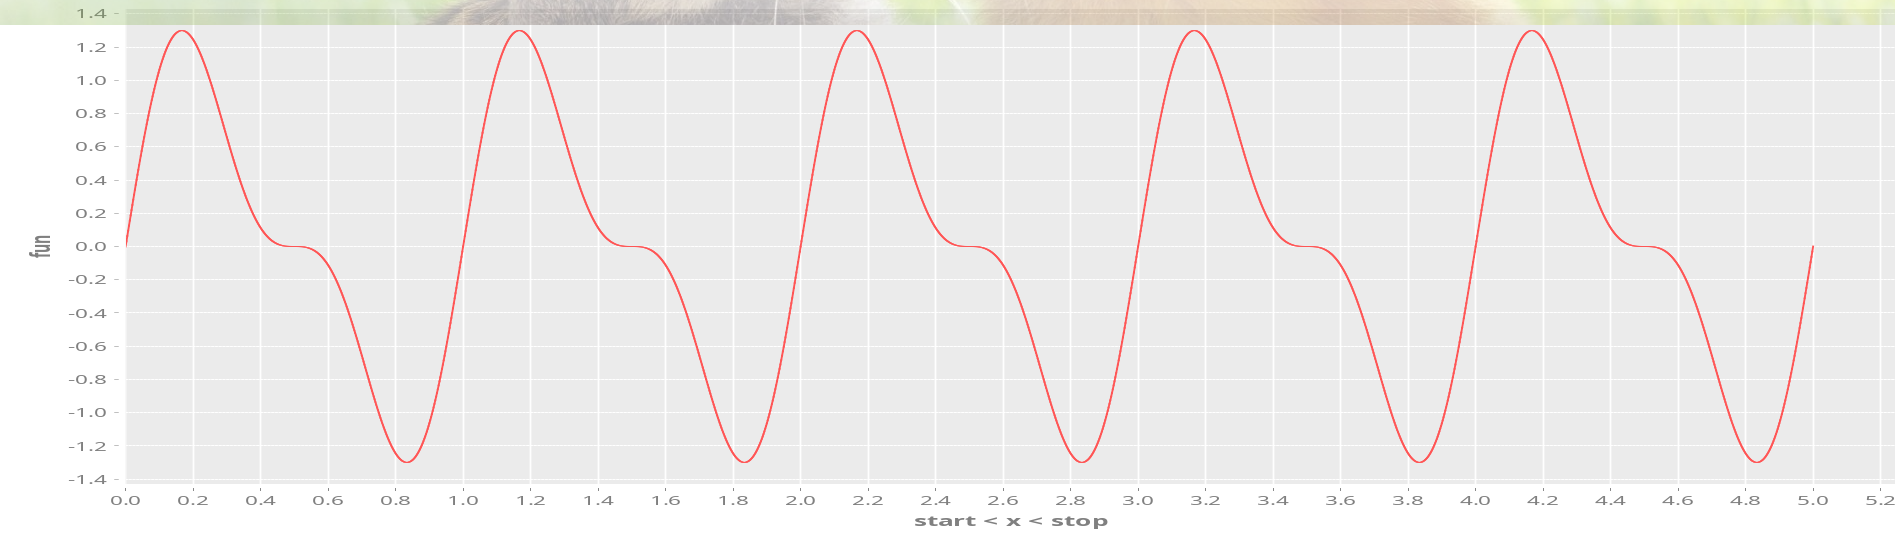
\includegraphics[width=\linewidth]{2a.png}
	\caption{funkcja $\sin x +\frac{\sin 2x}{2}$}
\end{figure}

\begin{figure}[H]
	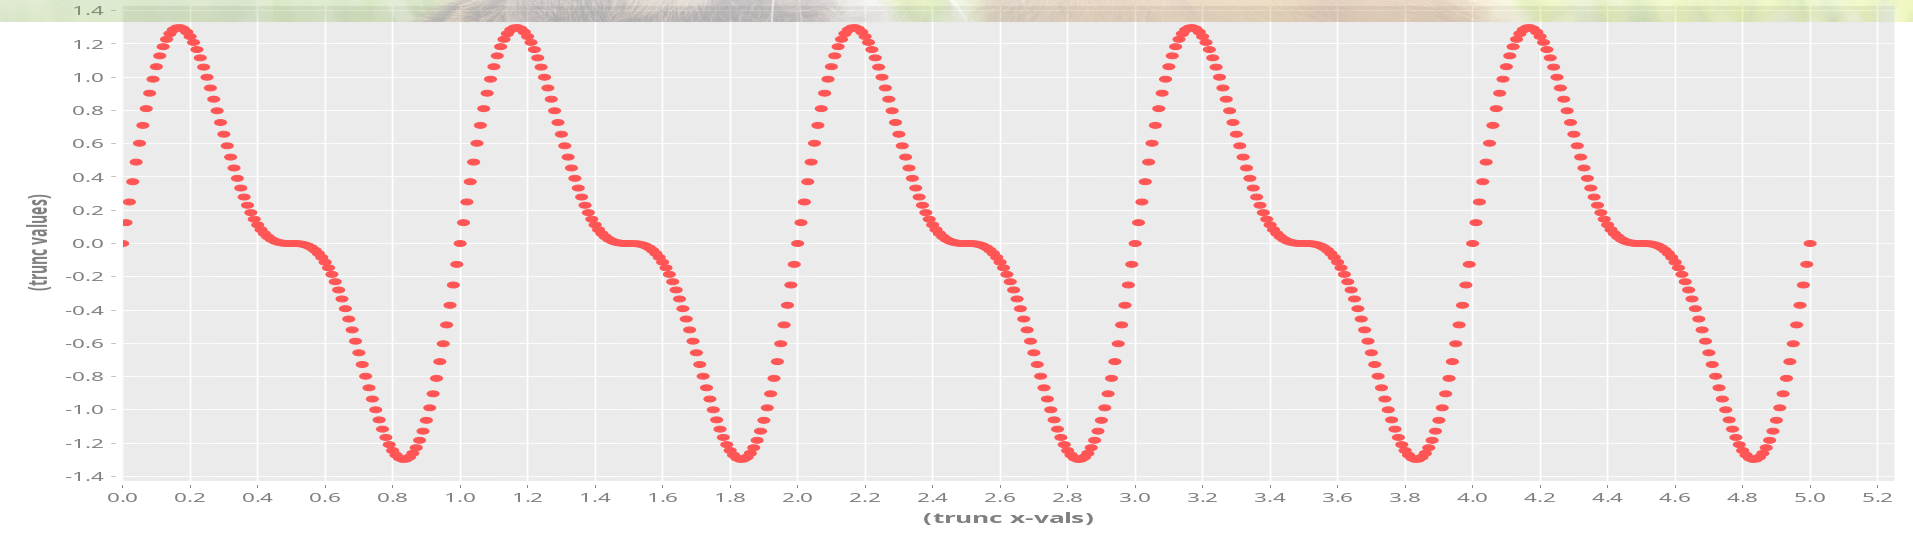
\includegraphics[width=\linewidth]{2a100.png}
	\caption{funkcja spróbkowana z częstotliwością 100Hz}
\end{figure}

\begin{figure}[H]
	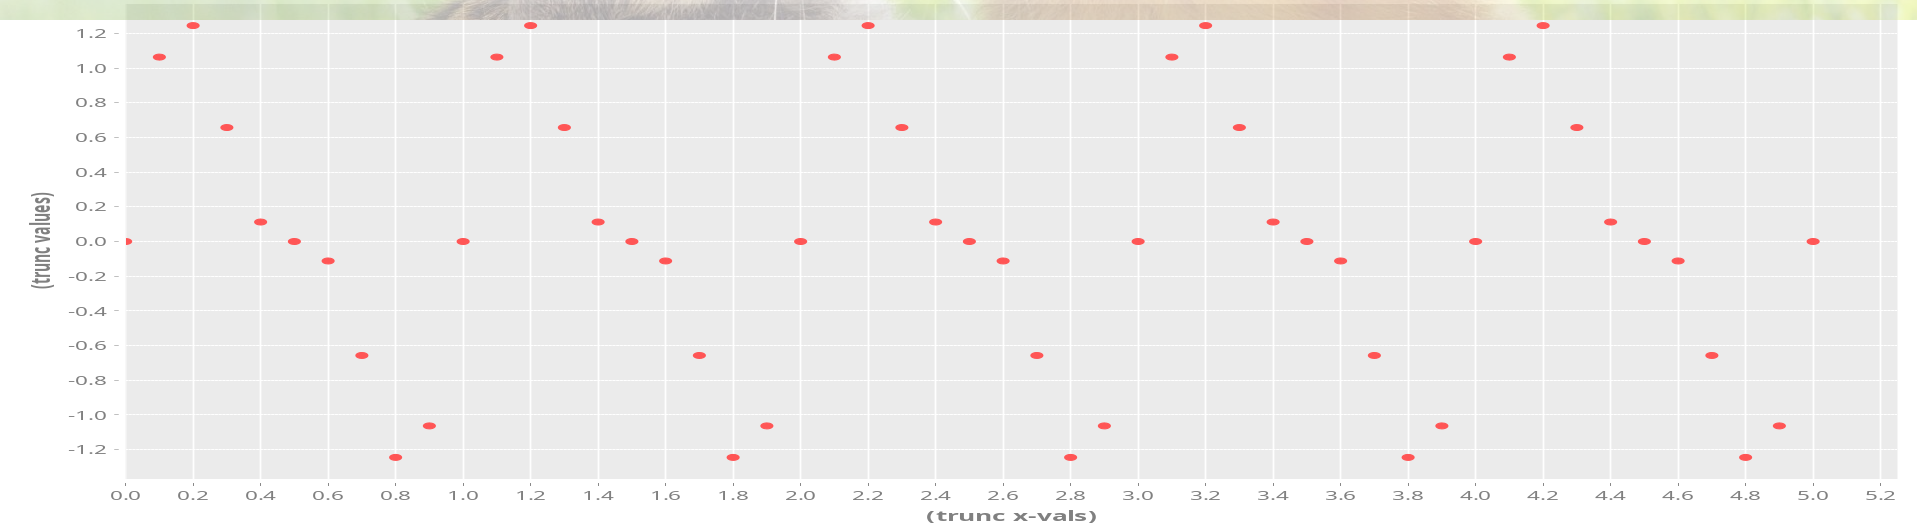
\includegraphics[width=\linewidth]{2a10.png}
	\caption{funkcja spróbkowana z częstotliwością 10Hz}
	\label{only}
\end{figure}

\subsection{kwantyzacja}
zastosowaliśmy kwantyzację z zaokrąglaniem


\begin{figure}[H]
	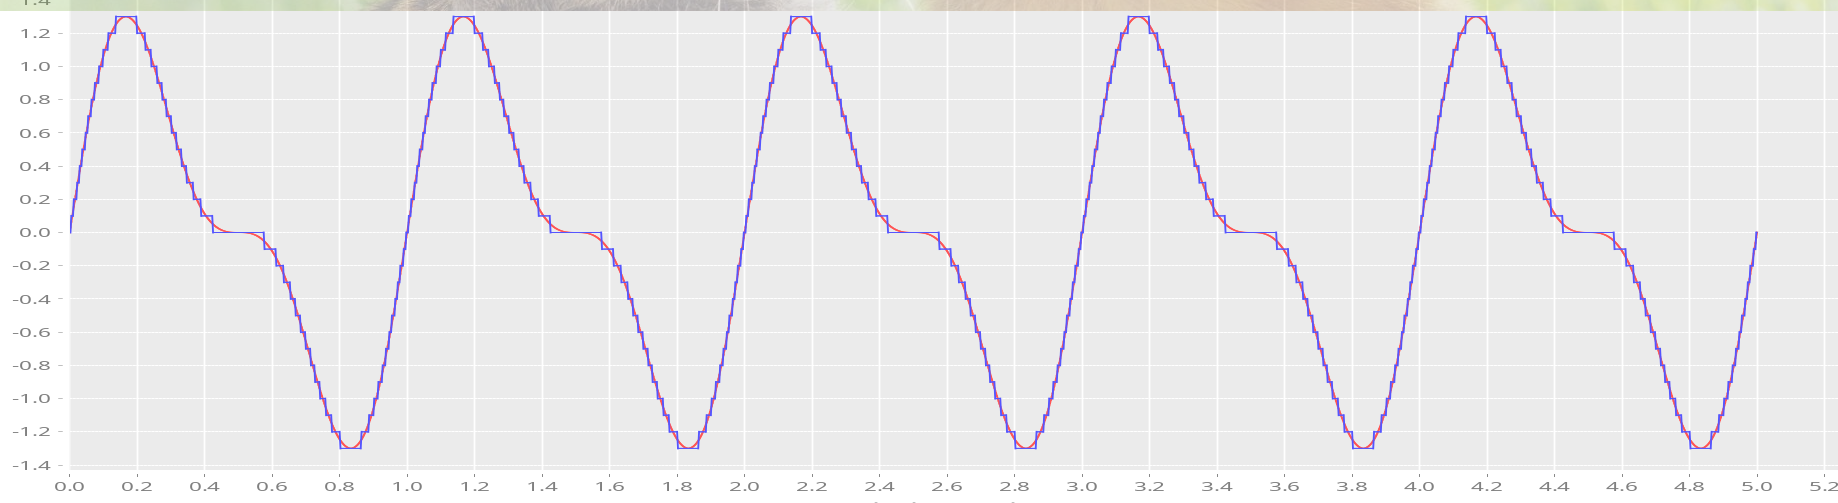
\includegraphics[width=\linewidth]{2akwant01.png}
	\caption{kwantyzacja z krokiem równym $0.1$}
\end{figure}


\begin{figure}[H]
	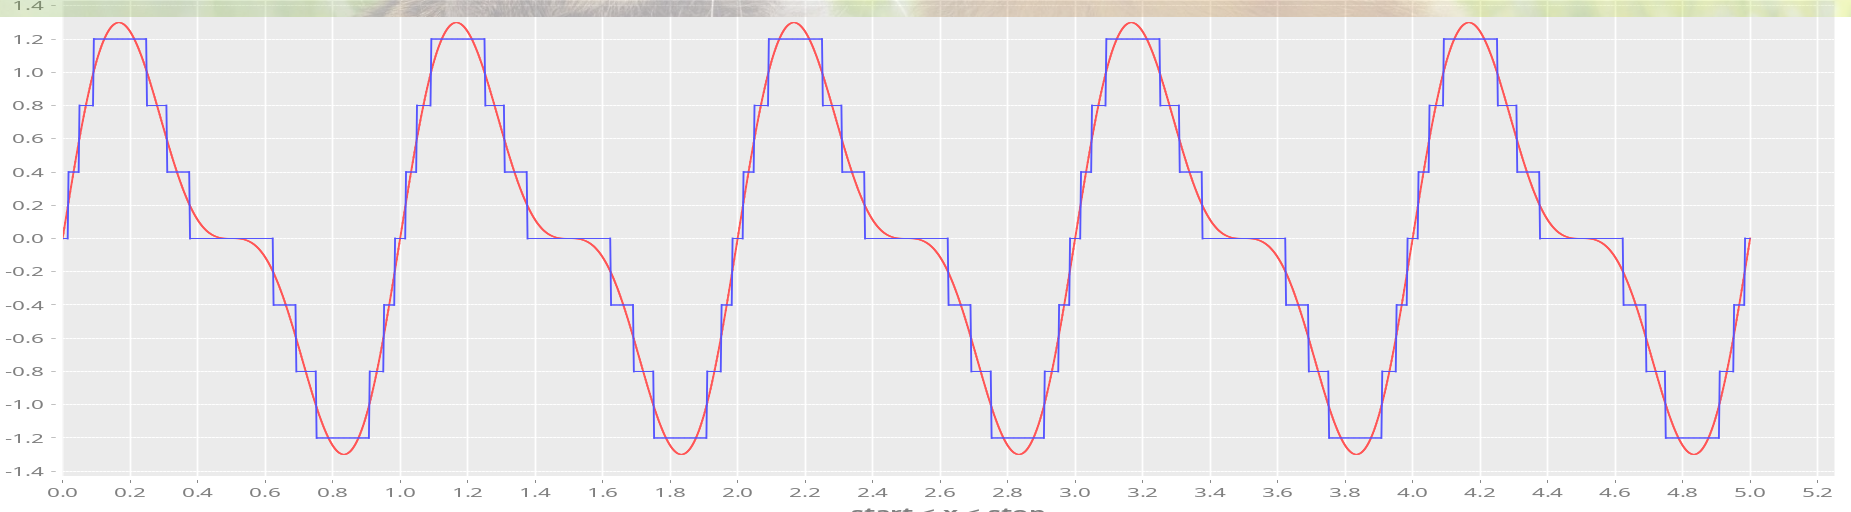
\includegraphics[width=\linewidth]{2akwant04.png}
	\caption{kwantyzacja z krokiem równym $0.4$}
\end{figure}

\begin{figure}[H]
	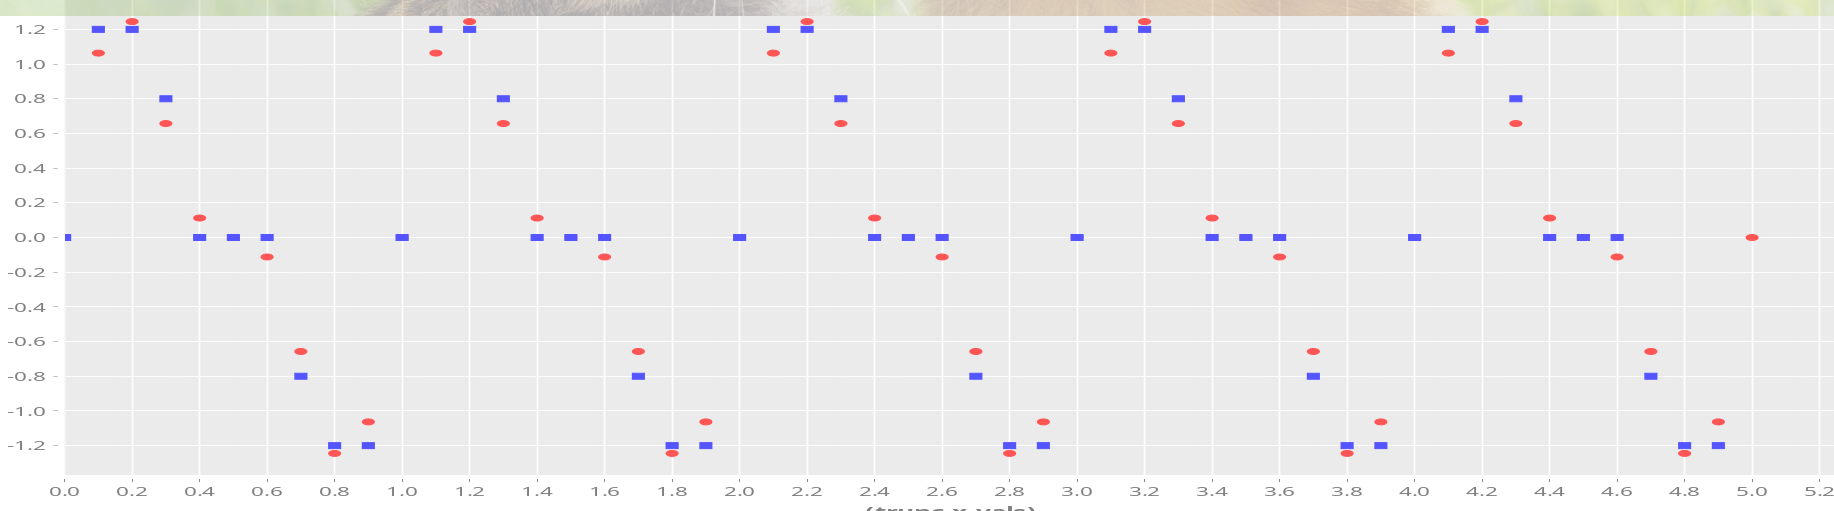
\includegraphics[width=\linewidth]{2aboth.png}
	\caption{kwantyzacja z krokiem równym $0.4$ i dyskretyzacja z częstotliwością 10Hz}
	\label{both}
\end{figure}


\subsection{interpolacja}

\begin{figure}[H]
	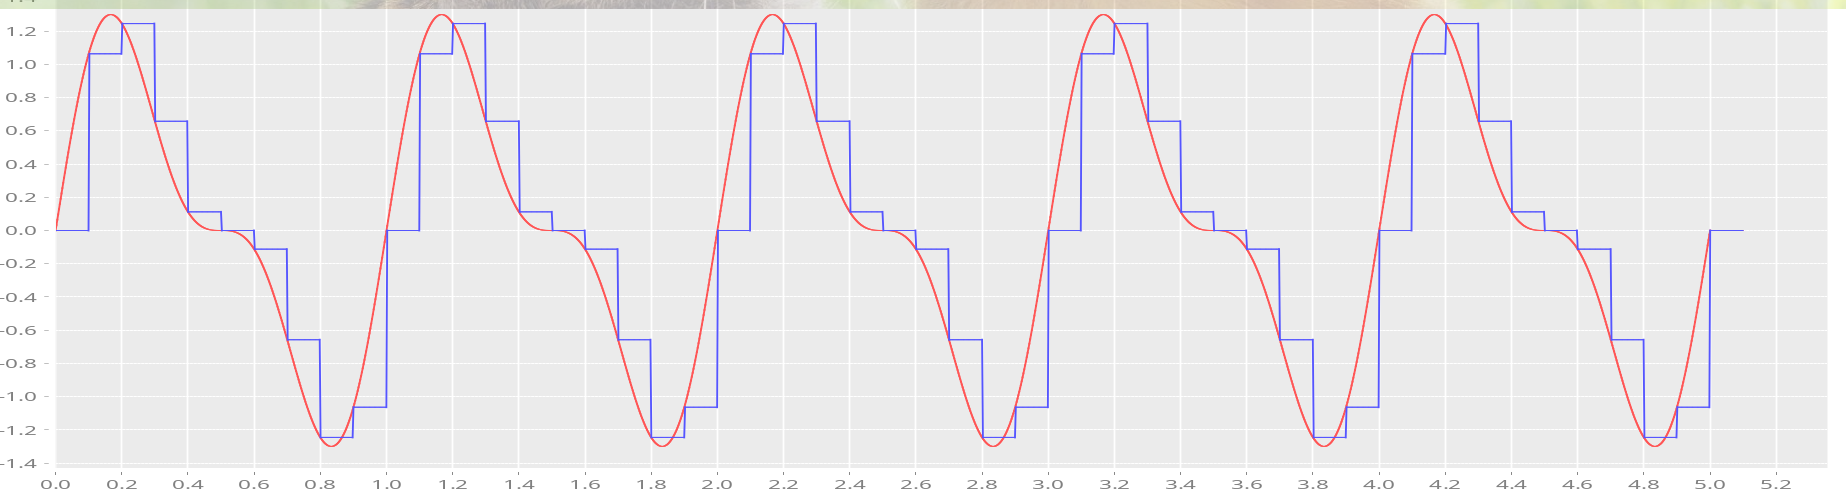
\includegraphics[width=\linewidth]{2z0.png}
	\caption{ekstrapolacja zerowego rzędu sygnału \ref{only}}
\end{figure}

\begin{figure}[H]
	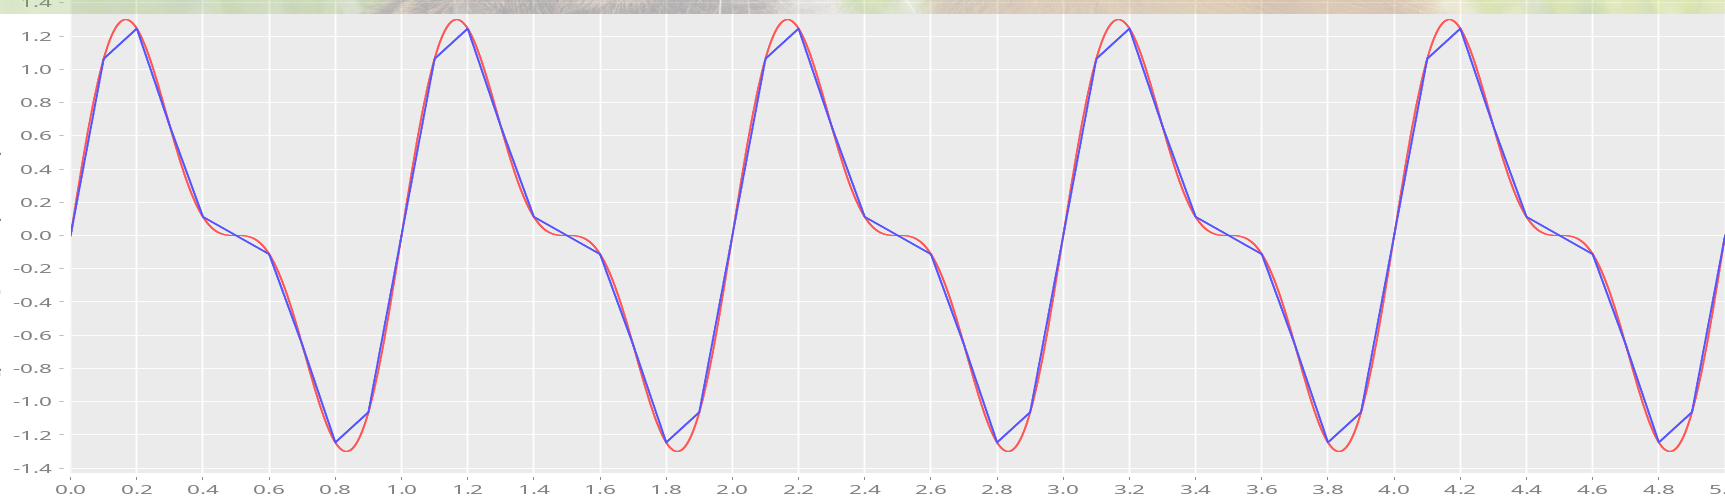
\includegraphics[width=\linewidth]{2z1.png}
	\caption{intprepolacja pierwszego rzędu sygnału \ref{only}}
\end{figure}

\begin{figure}[H]
	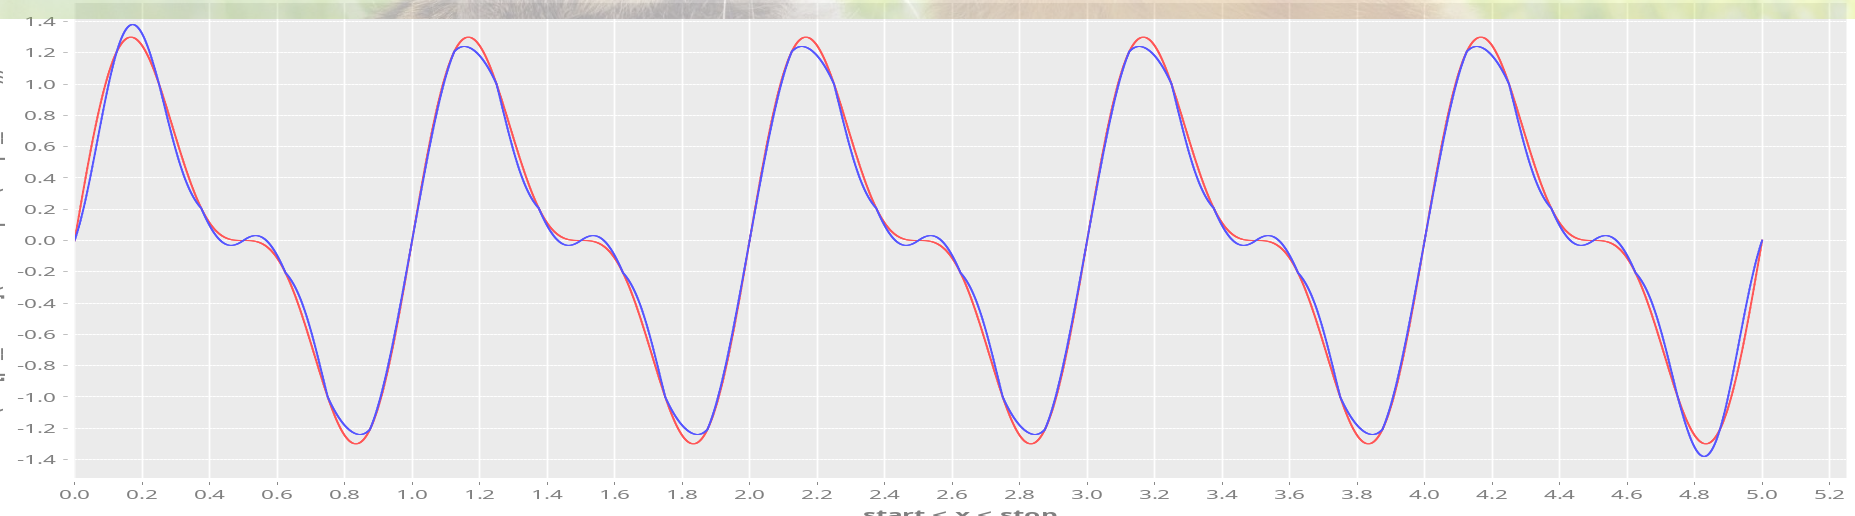
\includegraphics[width=\linewidth]{2zs3only.png}
	\caption{intprepolacja funkcją sinc sygnału \ref{only} dla n=3}
\end{figure}

\begin{figure}[H]
	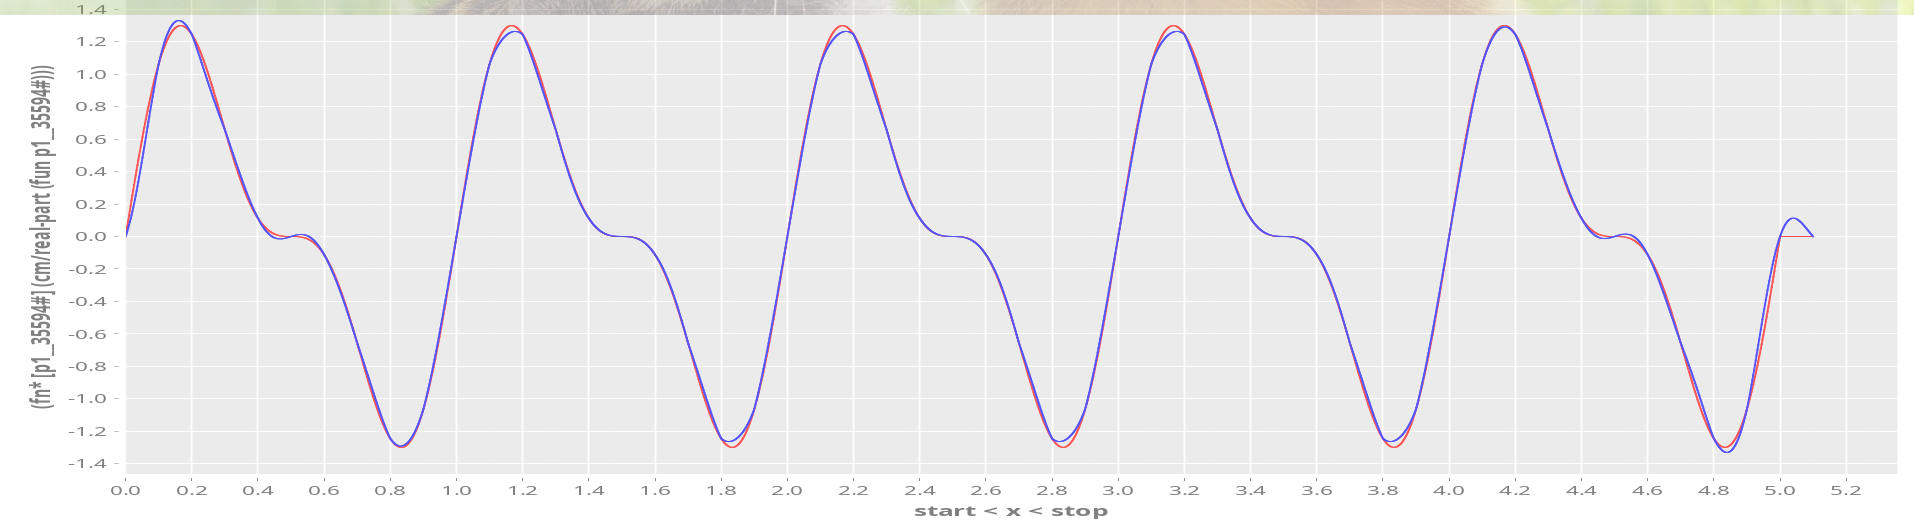
\includegraphics[width=\linewidth]{2zs10only.png}
	\caption{intprepolacja funkcją sinc sygnału \ref{only} dla n=10}
\end{figure}

\begin{figure}[H]
	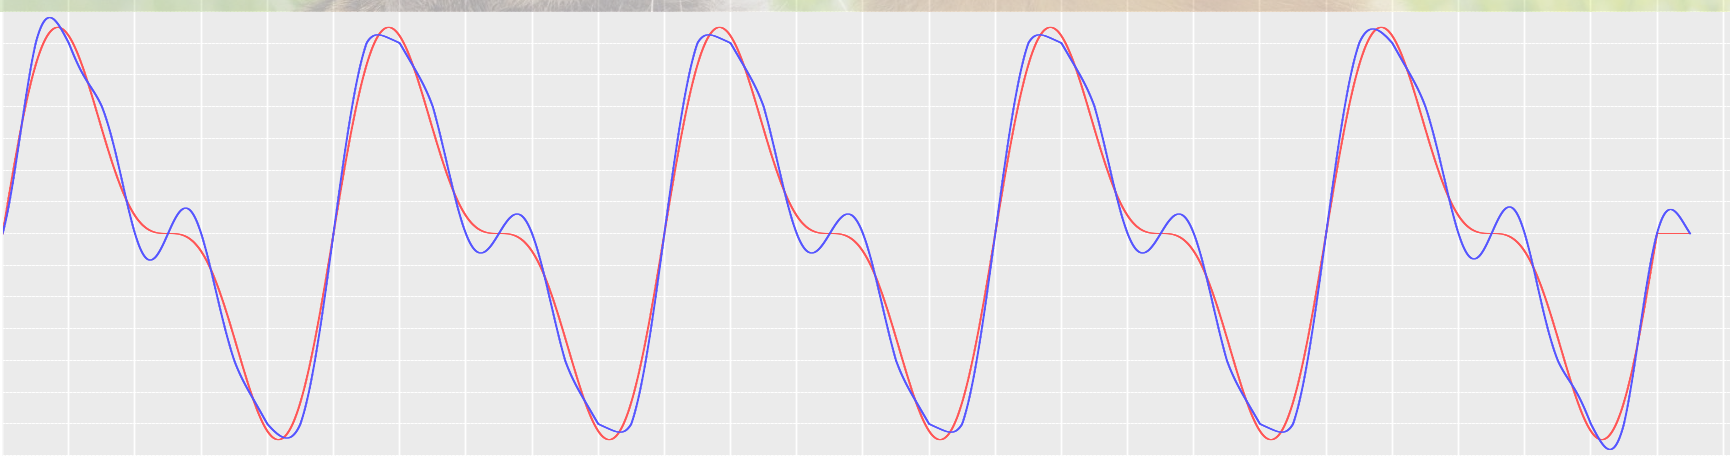
\includegraphics[width=\linewidth]{2zs10both.png}
	\caption{intprepolacja funkcją sinc sygnału \ref{both} dla n=10}
\end{figure}

\begin{table}[]
	\tiny
	\begin{tabular}{lllll}
		                 & MSE                    & PSNRDB              & SNRdb               & MD                   \\
		rzędu zerowego   & 0.0985150728915468,    & 10.06497316986428,  & 7.054673213224466,  & 0.7026499697988517   \\
		rzędu pierwszego & 0.0015432599731406956, & 28.115609077734717, & 25.105309121094905, & 0.0703770441156264   \\
		sinc dla n=3     & 5.357179910187408E-4,  & 32.71063768469473,  & 29.70033772805491,  & 0.04270139237439663  \\
		sinc dla n=10    & 5.999407676419332E-5,  & 42.21891625543191,  & 39.208616298792094, & 0.015900970476250165
	\end{tabular}
	\caption{błędy dla funkcji $\sin{x}$ (pomijając pierwszy i ostatni okres
		funkcji interpolowanej) dla częstotliwości próbkowania równej 8Hz}
\end{table}



\begin{table}[]
	\tiny
	\begin{tabular}{lllll}
		                 & MSE                   & PSNRDB             & SNRdb               & MD                  \\
		rzędu zerowego   & 0.17200816763660257,  & 7.644509305617029, & 4.634209348977215,  & 0.8639234171928447  \\
		rzędu pierwszego & 0.004776013609541633, & 23.2093444432835,  & 20.199044486643686, & 0.13397459621556196 \\
		sinc dla n=3     & 3.951938814533649E-4, & 34.03189787949822, & 31.02159792285841,  & 0.03964877422395152 \\
		sinc dla n=10    & 4.154473556817573E-5, & 43.81484000966347, & 40.80454005302366,  & 0.01841175521061783
	\end{tabular}
	\caption{błędy dla funkcji $\sin{x}$ (pomijając pierwszy i ostatni okres
		funkcji interpolowanej) dla częstotliwości próbkowania równej 6Hz}
\end{table}

\begin{table}[]
	\tiny
	\begin{tabular}{lllll}
		                 & MSE                    & PSNRDB             & SNRdb               & MD                    \\
		rzędu zerowego   & 0.3613823220289001,    & 4.420330959175279, & 1.4100310025354648, & 0.9999802608561372    \\
		rzędu pierwszego & 0.02276386418936745,   & 16.42754014083931, & 13.417240184199493, & 0.21051324277579175   \\
		sinc dla n=3     & 1.9311689484171246E-5, & 47.14179730282929, & 44.13149734618948,  & 0.0067737620416459254 \\
		sinc dla n=10    & 1.78102176919551E-4,   & 37.49330772179819, & 34.48300776515837,  & 0.04210653968767164
	\end{tabular}
	\caption{błędy dla funkcji $\sin{x}$ (pomijając pierwszy i ostatni okres
		funkcji interpolowanej) dla częstotliwości próbkowania równej 4Hz}
\end{table}


\begin{table}[]
	\tiny
	\begin{tabular}{lllll}
		                 & MSE                    & PSNRDB              & SNRdb                & MD                  \\
		rzędu zerowego   & 0.5857540838183046,    & 2.3228467486318545, & -0.6874532080079593, & 1.7299488209772846  \\
		rzędu pierwszego & 0.06608200970715618,   & 11.799167575845262, & 8.788867619205448,   & 0.4372561002186982  \\
		sinc dla n=3     & 4.5629794625681155E-4, & 33.407514859311334, & 30.397214902671518,  & 0.03832071760350286 \\
		sinc dla n=10    & 7.669638211644965E-4,  & 31.152251218909157, & 28.141951262269345,  & 0.08417439352790212
	\end{tabular}
	\caption{błędy dla funkcji $\sin{x}$ (pomijając pierwszy i ostatni okres
		funkcji interpolowanej) dla częstotliwości próbkowania równej 3Hz}
\end{table}

dla częstotliwości równej 2Hz wszystkie próbki łaimy amplitudę równą 0.











%%%%%%%%%%%%%%%%%%%%%%%%%%%%%%%%%%%%%%%%%%%%%%%%%%%%%%%%%%%%%%%%%%%%%%%%%%%%%%%%%%%%%%%%%%%%%%%%%%%%%%%%%%%%%%%%%
% PODROZDZIA\xC5\x81 PT. ZALACZNIKI
%%%%%%%%%%%%%%%%%%%%%%%%%%%%%%%%%%%%%%%%%%%%%%%%%%%%%%%%%%%%%%%%%%%%%%%%%%%%%%%%%%%%%%%%%%%%%%%%%%%%%%%%%%%%%%%%%
%%%%%%%%%%%%%%%%%%%%%%%%%%%%%%%%%%%%%%%%%%%%%%%%%%%%%%%%%%%%%%%%%%%%%%%%%%%%%%%%%%%%%%%%%%%%%%%%%%%%%%%%%%%%%%%%%
% BIBLIOGRAFIA
%%%%%%%%%%%%%%%%%%%%%%%%%%%%%%%%%%%%%%%%%%%%%%%%%%%%%%%%%%%%%%%%%%%%%%%%%%%%%%%%%%%%%%%%%%%%%%%%%%%%%%%%%%%%%%%%%
\cite{instrukcja}
\renewcommand\refname{Bibliografia}
\bibliographystyle{plain}
\bibliography{ich}

\end{document}
